\documentclass[a4paper, 11pt]{article}
% TeX-template
% Copyright (c) 2024 Joseph Tooby-Smith. All rights reserved.
% Released under Apache 2.0 license.
% Paper content: 
% Copyright (c) 2024 Joseph Tooby-Smith. All rights reserved.
\usepackage{xcolor}
\usepackage{setspace}

\onehalfspacing%
%\setstretch{3} % Custom separation of lines.
\renewcommand{\arraystretch}{1.5}
%%%%%%%%%%%%%%%%%%%%%%%%%%%%%%%%
%Hyperlinks
\usepackage{hyperref}
\definecolor{mycolor}{RGB}{0,88,204}
\hypersetup{
  colorlinks=true,
  linkcolor=mycolor,
  urlcolor=mycolor,
  citecolor=mycolor
}
%%%%%%%%%%%%%
%Watermark
\usepackage{draftwatermark}
\SetWatermarkText{\color{mycolor} DRAFT}
\SetWatermarkScale{1.5}
%%%%%%%%%%%%%%%%%%%%%%%%%%%%%%%%
%Mathematics
\usepackage{amsmath}
%%%%%%%%%%%%%%%%%%%%%%%%%%%%%%%%
%Margins
\usepackage{geometry}

\geometry{
  top=0.8in,
  bottom=0.8in,
  left=1in,
  right=1in
}
%%%%%%%%%%%%%%%%%%%%%%%%%%%%%%%%
%Page numbers
\usepackage{fancyhdr}


\pagestyle{fancy}
\fancyhf{}
\fancyhead[R]{\thepage}
\renewcommand{\headrulewidth}{0pt}
\setlength{\headheight}{13.6pt}
%For the title page
\fancypagestyle{plain}{%
  \fancyhf{}
  \fancyhead[R]{\thepage}
  \renewcommand{\headrulewidth}{0pt}
}
%%%%%%%%%%%%%%%%%%%%%%%%%%%%%%%%
%Fonts

\usepackage{mathptmx}

%%%%%%%%%%%%%%%%%%%%%%%%%%%%%%%%
%Section style

\usepackage{titlesec}

\titleformat{\section}
  {\normalfont\large\centering}{\thesection.}{1em}{\MakeUppercase}
\titleformat{\subsection}
  {\normalfont\centering}{\thesubsection.}{1em}{\MakeUppercase}

  \titlespacing{\paragraph}{10pt}{0pt}{6pt}[0pt]
%%%%%%%%%%%%%%%%%%%%%%%%%%%%%%%%
%Comments

\newcommand{\js}[1]{ {\color{magenta} js:  #1}}

%%%%%%%%%%%%%%%%%%%%%%%%%%%%%%%%
%SVG images
\usepackage{svg}
%%%%%%%%%%%%%%%%%%%%%%%%%%%%%%%%
%Paragraph markers
%\newcommand{\paragraphMarker}[1]{ %{\color{gray} $\langle$#1$\rangle$}
%}
%%%%%%%%%%%%%%%%%%%%%%%%%%%%%%%
%Lean formating
\usepackage{listings}
\usepackage[T1]{fontenc}
\usepackage[utf8]{inputenc}
\usepackage{amssymb}
\usepackage{chngcntr}
\definecolor{keywordcolor}{rgb}{0.7, 0.1, 0.1}   % red
\definecolor{tacticcolor}{rgb}{0.0, 0.1, 0.6}    % blue
\definecolor{commentcolor}{rgb}{0.4, 0.4, 0.4}   % grey
\definecolor{symbolcolor}{rgb}{0.0, 0.1, 0.6}    % blue
\definecolor{sortcolor}{rgb}{0.1, 0.5, 0.1}      % green
\definecolor{attributecolor}{rgb}{0.7, 0.1, 0.1} % red

\def\lstlanguagefiles{lstlean.tex}
\lstset{
 	frame = lrtb,
 	rulecolor=\color{mycolor},
	language=lean,
	aboveskip = 5mm,
	belowskip = 5mm,
	captionpos=t
	}

\lstnewenvironment{code}[1][]%
{
   \noindent\newline
   \minipage{\linewidth}
   \vspace{0.5\baselineskip}
   \lstset{
 	frame = lrtb,
 	rulecolor=\color{mycolor},
 	escapeinside={/*!}{!*/},
	language=lean,
	aboveskip = 5mm,
	belowskip = 5mm,
	xleftmargin=2mm,
	xrightmargin=2mm,
	}
	}
{\endminipage\newline}
\lstnewenvironment{codeLong}[1][]%
{
   \lstset{
 	frame = lrtb,
 	rulecolor=\color{mycolor},
 	escapeinside={/*!}{!*/},
	language=lean,
	aboveskip = 5mm,
	belowskip = 5mm,
	xleftmargin=2mm,
	xrightmargin=2mm,
	}
	}
{}
%%%%%%%%%%%%%%%%%%%%%%%%%%%%%%%%
%Links in code block
% put at top of code block using
% /*!\codeLink{...}!*/
\newcommand{\codeLink}[1]{
  \vspace{-0.5cm}\hfill\href{https://github.com/HEPLean/HepLean/blob/1b951994ae3d882242b02d23957ef1ee7fa05f3d/HepLean/#1}{(source)}
  }
  \newcommand{\codeBreakdownLink}[2]{
  \vspace{-0.5cm}\hfill\href{https://github.com/HEPLean/HepLean/blob/1b951994ae3d882242b02d23957ef1ee7fa05f3d/HepLean/#1}{(source)}
  (breakdown \ref{#2})
  }
 \newcommand{\textLink}[1]{\href{https://github.com/HEPLean/HepLean/blob/1b951994ae3d882242b02d23957ef1ee7fa05f3d/HepLean/#1}{source}}
 \newcommand{\textLinkB}[1]{\href{https://github.com/HEPLean/HepLean/blob/1b951994ae3d882242b02d23957ef1ee7fa05f3d/HepLean/#1}{(source)}}
%%%%%%%%%%%%%%%%%%%%%%%%%%%%%%%%
%Title, author, date
\title{Index notation in Lean 4}
\author{Joseph Tooby-Smith \\ \textit{Reykjavik University}}
\date{\today}
%%%%%%%%%%%%%%%%%%%%%%%%%%%%%%%%

\begin{document}
\counterwithin{lstlisting}{section}
\maketitle
\vspace{-1cm}
\begin{abstract}
The physics community relies on index notation to effectively manipulate tensors of specific 
types. This paper introduces the first formally verified implementation of index notation in the
interactive theorem prover Lean 4. By integrating index notation into Lean, we bridge the gap between 
traditional physics notation and formal verification tools, 
making it more accessible for physicists to write and prove results within Lean.
In the background, our implementation leverages a novel application of category theory.
\end{abstract}

\section{Introduction}

\paragraph{HepLean} In previous work, the author initiated the formalization of high energy physics 
results using the interactive theorem prover Lean 4 in a project called HepLean. 
Lean is an interactive theorem prover and 
programming language with syntax resembling traditional pen-and-paper mathematics. 
Lean allows users to write definitions, theorems, and proofs 
which are then automatically checked, using its foundation of dependent-type theory, for correctness.
HepLean has four main motivations: \js{sorry}

\paragraph{Other works in Lean} HepLean is part of a broader movement of projects
to formalize parts, or all, of 
mathematics and science. The largest of these projects is Mathlib, which aims to formalize
mathematics. Indeed, HepLean is built downstream of Mathlib, meaning it has Mathlib as a 
dependency and uses many of the definitions and theorems from there. 
Other projects include the ongoing effort led by Kevin Buzzard to formalize the proof of Fermat's
Last Theorem into Lean. 
In the realm of the sciences, \js{sorry}

\paragraph{Notation in physics and index notation:}
Physicists heavily rely on specialized notation to express complex concepts succinctly. 
Among these, index notation is particularly prevalent,
 as it provides a compact and readable way to represent specfic types of tensors and operations
 between them.

\paragraph{Challange:} Formalizing index notation into an interactive theorem prover like Lean 
is chalanging due to the complexity and implicitness 
of the notation and the need for flexiable  and rigour in it's formalization. 
This paper presents such an implementation of index notation within the HepLean project.


\paragraph{Motivation:} The primary motivations for implementing index notation into Lean are:
\begin{enumerate}
  \item To make easier to write and prove results from high energy physics into Lean. 
  \item To make the syntax of Lean more familiar to high energy physicists use to index notation.
\end{enumerate}
We hope that the implementation  of index notation into Lean
not only enhances usability but also promotes the adoption of formal methods in the 
physics community.

\paragraph{Conclusion:} The conclusion of the implentation of index notation into Lean 4 is that 
we can write results like the following: 
\begin{equation}
\js{Add example}
\end{equation}
and lean will correctly intpret this result as a formal mathematical object which proves can be 
applied to.


\paragraph{Other papers:}
Previous attempts to formalize index notation have been made in programming languages like Haskell 
\cite{haskell-index-notation}. However, these implementations do not
 provide the formal verification capabilities inherent in Lean. 
 The formal verification requirement of Lean introduces unique challenges in implementing index 
 notation, necessitating (what we beleive is) a novel solution.


\paragraph{Outline:} This paper is split into two main sections. Section \js{ref} dicusses 
the implementation of index notation into Lean. Section \js{ref} gives two examples 
of theorems and proofs using index notation. A more minor section, section \js{ref} disucsses 
the future work related to this project.


\section{Implementation of index notation into Lean 4}
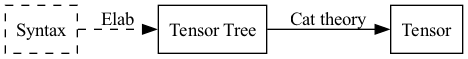
\includegraphics[width=\textwidth]{overviewFlow.png}
The implementation of index notation in Lean can be  broken down into 
three main components, illustrated in Figure \js{ref}. 
The first component is the \emph{syntax for tensor expressions}, 
which is what users interact with when writing results in Lean. 
This syntax closely mirrors the notation familiar to physicists, 
making it intuitive and accessible. 
It appears directly in the Lean files and can be thought of as an informal string 
that represents the tensor expressions.

The second component involves transforming this syntax into a \emph{tensor tree}. 
The tensor tree is a formal mathematical representation of the tensor expression. 
By parsing the informal syntax into a structured tree, 
we establish a rigorous foundation that captures the tensor expression. 
This formal representation allows us to easily manipulate tensor expressions and
prove results related to them in a way that Lean accepts as formal.

The third and final component is the conversion of the tensor tree into an actual \emph{tensor}. 
This process utilizes properties of the symmetric-monoidal category of representations
 to translate the abstract tensor tree into a concrete tensor.

These three steps—syntax, tensor tree, and tensor—are illustrated in Figure \js{ref}. 
Although Lean processes information from left to right, 
starting with the syntax and proceeding to the tensor tree, and then finally (when 
we ask it to) to the tensors, 
it is more effective to discuss the implementation from right to left. 
This reverse approach is advantageous because the tensors,
 which are the primary objects of interest, are located on the right side of the diagram. 
 The left and middle parts of the diagram represent intermediate stages that facilitate the 
 manipulation and understanding of these tensors and their expressions.

 \subsection{Defining tensors}

\subsubsection{Building blocks of tensors and color}

Tensors of a species, such as complex Lorentz tensors, are constructed from a 
set of building block representations of a group $G$ over a field $k$.
For complex Lorentz tensors, the group $G$ is $SL(2, \mathbb{C})$, the field $k$ is the 
field of complex numbers. 

There are six building block representations for complex Lorentz tensors. These are
\begin{itemize}
  \item \lstinline|Fermion.leftHanded| is the
   representation of $SL(2, \mathbb{C})$ corresponding 
      $v \mapsto M v$, corresponding to Left-handed Weyl fermions.
  \item \lstinline|Fermion.altLeftHanded| is the
  representation of $SL(2, \mathbb{C})$ corresponding 
     $v \mapsto M^{-1 T} v$, corresponding to alternative Left-handed Weyl fermions (as we will 
     call them).
  \item \lstinline|Fermion.rightHanded| is the representation of $SL(2, \mathbb{C})$ corresponding 
  $v \mapsto M^\star v$, corresponding Right-handed Weyl fermions.
  \item \lstinline|Fermion.altRightHanded| is the representation of $SL(2, \mathbb{C})$ corresponding
  $v \mapsto M^{-1 \dagger} v$, corresponding to alternative Right-handed Weyl fermions.
  \item \lstinline|Lorentz.complexContr| is the representation of $SL(2, \mathbb{C})$ 
   induced by the homomorphism of $SL(2, \mathbb{C})$ into the Lorentz group and the contravariant 
   action of the Lorentz group on four-vectors
  \item \lstinline|Lorentz.complexCo| is the representation of $SL(2, \mathbb{C})$
    induced by the homomorphism of $SL(2, \mathbb{C})$ into the Lorentz group and the covariant
    action of the Lorentz group on four-vectors.
\end{itemize}
As an example the representation \lstinline|Fermion.leftHanded| is defined in Lean as follows:
\begin{code}
def leftHanded : Rep ℂ SL(2,ℂ) := Rep.of {
    toFun := fun M => {
      toFun := fun (ψ : LeftHandedModule) =>
        LeftHandedModule.toFin2ℂEquiv.symm (M.1 * ψ.toFin2ℂ),
      map_add' := by
        intro ψ ψ'
        simp [mulVec_add]
      map_smul' := by
        intro r ψ
        simp [mulVec_smul]}
    map_one' := by
      ext i
      simp
    map_mul' := fun M N => by
      simp only [SpecialLinearGroup.coe_mul]
      ext1 x
      simp only [LinearMap.coe_mk, AddHom.coe_mk, LinearMap.mul_apply, LinearEquiv.apply_symm_apply,
        mulVec_mulVec]}  
\end{code} \js{Not exact definiton as could not type $*\_v$}
Here the  outer \lstinline|toFun| argument is defining a map from $SL(2,\mathbb{C})$ to linear maps 
from \lstinline|LeftHandedModule| (equivalent to $\mathbb{C}^2$) to itself. The inner \lstinline|toFun|, 
\lstinline|map_add'| and \lstinline|map_smul'| are defining defining respectively, the underlying 
function of this linear map, and proving it it linear with respect to addition and scalar multiplication.
The \lstinline|map_one'| and \lstinline|map_mul'| are proving that action of the identity is trivial, 
and that the action of the product of two elements is the product of the actions of the elements.

We assign a unique label, which we refer to as a \emph{color}, to each of the 
building block representations. We denote the type of colors for a given species of tensors as $C$.
For complex Lorentz tensors 
$C$ is defined as 
\begin{code}
inductive Color
  | upL : Color
  | downL : Color
  | upR : Color
  | downR : Color
  | up : Color
  | down : Color
\end{code}
Here \lstinline|Color| is the name of our type and \lstinline|upL|, \lstinline|downL|, etc. are the
colors. 

To formally associate each color with its corresponding representation, we define
a discrete functor from the set $C$ to the category of $k$-representations of $G$, denoted 
$\mathrm{Rep} k G$, that is, a functor
\begin{equation} 
  F_{D} : C \Rightarrow \mathrm{Rep} k G.
\end{equation}


For complex Lorentz tensors this functor in Lean as follows:
\begin{code}
FDiscrete := Discrete.functor fun c =>
  match c with
  | Color.upL => Fermion.leftHanded
  | Color.downL => Fermion.altLeftHanded
  | Color.upR => Fermion.rightHanded
  | Color.downR => Fermion.altRightHanded
  | Color.up => Lorentz.complexContr
  | Color.down => Lorentz.complexCo
\end{code}

The reason why we have used a functor here, rather than just a function, will become apparent
in what follows.


\subsubsection{A general tensor}

For a given tensor species, given the symmetric monoidal structure on $\mathrm{Rep} k G$, 
we can take the tensor product of the building block representations. 
Elements of such tensor products form the general notion of a tensor for that given 
species. 

To formalize this in Lean, we consider the category  $\mathcal{S}_{/C}^\times$. The objects 
of $\mathcal{S}_{/C}^\times$ are functions $f : X \to C$  for some type $X$. 
A morphism from $f : X \to C$ to $g : Y \to C$ is a bijection $\phi : X \to Y$ such that 
$f = g \circ \phi$. 
This category is equivalent to the core of the category of types ($\mathcal{s}$) over $C$, hence 
our notation. 

Any functor $H : C \Rightarrow \mathrm{Rep} k G$ can be lifted to a symmetric monoidal 
functor $\mathcal{S}_{/C}^\times \Rightarrow \mathrm{Rep} k G$ which takes $f$ to the 
tensor product $\bigotimes_{x \in X} H(f(x))$ and morphisms to the linear maps 
of representations corresponding to reindexings of
tensor products.

This construction is itself functorial, 
giving a functor: 
\begin{equation}
  \mathrm{lift} : \mathrm{Fun}(C, \mathrm{Rep} k G) \Rightarrow
  \mathrm{SymmMonFun}(\mathcal{S}_{/C}^\times, \mathrm{Rep} k G)
\end{equation} 
In the previous subsection we defined the functor $F_{D}$ which associates to each color 
its corresponding representation. We can then define a functor $F$ by the image of $F_{D}$ under
the lift functor. 

A tensor of a given species can then be thought of as a vector in the representations in the of $F$.
Defining a tensor in this way allows us to utalize the 
structur of monodial categories and functors in a useful way. 

In HepLean we formally define $\mathrm{lift}$ and $F$. 

For most purposes in physics $X$ will be a type $\mathrm{Fin} n$, corresponding to the type 
(set) of natural numbers (including 0) less $n$. Later on we will restrict to these types.

\subsubsection{Basic operations}

Now we have discussed how tensors of a given species can be formally defined, we can define 
basic operations on these tensors. 

With the exception of evaluation, all the operations we perform on tensors comes from one of four 
place. From the definition of a vector space and a representation, 
from the monoidal structure of the categories and functors involved, the functor $F$ itself
or from morphisms in $\mathrm{Fun}(C, \mathrm{Rep} k G)$. 

\paragraph{Operations from the representations:} These are the simplist operations one can perform 
on a tensor. For $f : X \to C$ an object in $\mathcal{S}_{/C}^\times$ we can add two tensors 
in $F(f)$, multiply a tensor in $F(f)$ by a element of $k$, or use the representation 
of $G$ on $F(f)$ to act with $G$ on a tensor in $F(f)$. 

\paragraph{Operations from the monoidal structure:} The monoidal structure of the category of 
representations gives us the tensor product of two tensors. 
Given $f : X \to C$ and $g : Y \to C$, and tensors $t \in F(f)$ and $s \in F(g)$ we can form
a tensor $t \otimes s \in F(f) \otimes F(g)$\footnote{\js{One can think of this as taking the tensor product of morphisms $\mathbb{1} \to F(f)$ and $\mathbb{1} \to F(g)$.}} \js{make sure defined monoidal structure on $\mathcal{S}_{/C}^\times$}. 
Since $F$ is a symmetric monoidal functor we get a morphism from $F(f) \otimes F(g) \to F(f \otimes g)$. 
Thus we can form a new tensor $t \otimes s \in F(f \otimes g)$.

\paragraph{Operations from the functor $F$:} The functor $F$ itself gives us 
the ablity to permute indices of a tensor.

\js{More to write here.}

\begin{itemize} 
\item The formalisim we have discribed thus far gives us basic oprations on tensors for free.
\item We get addition, scalar multiplication and the action of the group $SL(2, \mathbb{C})$ from 
  the fact that things sit in representations. 
\item We also get the tensor product of two tensors, from the category of representations 
  and the fact that our lift function is symmetric monoidal. 
\item We get permutation of indices from the fact we have a functor. 
\item We get negation of tensors because \js{sorry}
\item We also get the interplay between all of these
\item There somethings we do not get for free however: Contraction, the unit of the contraction, 
  and the metrics. 
\item To define these we need introduce an involution $\tau : C \to C$. We will call the image of 
  $c$ under $\tau$ the dual of $c$.
\item Colors can be self-dual, as there for Einstein tensors, for which there is only one color. 
\item From $\tau$ we get a functor $\tau_* : \mathcal{S}_{/C}^\times \to \mathcal{S}_{/C}^\times$.
\item We let $F_\tau$ be the functor from $C$ to $F(c) \otimes F(\tau c)$.
\item To define contraction we define a natural transformation $ F_\tau \to \mathbb{1}$.
\item That is for each $c$ a morphism of representations from   $F(c) \otimes F(\tau c)$ to the 
  trivial representation.
\item To give an example for complex Lorentz tensors \js{sorry}
\item Using $F_\tau$ we can contract indices of tensors of dual colors. 
\item Lifiting $F_\tau$ gives us a functor which would allow us to contract all indices of a tensor
 at ones. This may be useful for come computations. 
\item In addition to contraction we want the notion of a metric.  
\item \js{Unit}
\item  \js{Conditions}
\end{itemize}

\subsubsection{Tensor Species}

\begin{itemize}
  \item The data we have given so far consitutes what we have losely being calling a Tensor species. 
  \item In Lean we make this more precise 
\end{itemize}

\subsection{Tensor trees}
\subsubsection{Structure}
\begin{itemize}
  \item A tensor expression consists of a series of tensors and operations performed on them. 
  \item We can represent such an expression using a tensor tree, similar to the notion of a 
    syntax tree.
  \item A tensor tree has different types of nodes either representing a tensor or a operation 
    on or between tensors. 
  \item Since we really only care about tensors with $X = Fin n$, tensor trees in Lean are 
    implemented only for these. 
  \item Let us give the definition of a tensor tree and then dicuss in turn each of the nodes. 
  \item \js{Lean defn of tensor tree}
  \item The basic node is a tensor node. The definition in Lean tells us how this is defined. 
  \item Then for each operation addition, scalar mult, group action etc. we get a node. 
  \item For example let us look at contraction 
  \item \js{sorry}
  \item How we turn these tensor trees into tensors will be dicussed in the next section
\end{itemize}

\subsubsection{To a tensor}

\begin{itemize}
  \item The notion of a tensor tree is defined without reference to the category theory 
    we have been discussing. 
  \item We can however turn a tensor tree into a tensor using said constructions. 
  \item The definition of how we do this is defined recursively. 
\end{itemize}

\subsubsection{Using Tensor trees in proofs}
\begin{itemize}
  \item \js{Discuss fact about `tensor\_eq'}
\end{itemize}
\subsection{Elboration}
\begin{itemize}
  \item We have dicussed the implementation of tensor species into Lean, and how to write
    tensor expressions using tensor trees.
  \item Really this is all one needs to effectively. 
  \item However, we want our theorems to look like they do on paper. 
  \item This is the role of the elaborator, which here takes a string written in lean code 
    and turns it into a tensor tree.
  \item It is perhpase easist to give examples: 
  \item The basic notation for a tensor nodes is \js{sorry}. Note that ... are free indices, 
    it does not matter what we call them the expression is the same. 
  \item The product of two tensors is written as \js{sorry}.
  \item The contraction of two tensors is written as \js{sorry}. Again note that the indices 
    are free so we can call them anything without chaning how lean reads the expression. 
  \item We also define a special notation of equality and addition. which takes account of permutation.
  \item This part of the Lean code is not formally verified, it is just telling lean how to 
    read the notation. Once the tensor tree is created and we start using that, things are formally 
    verifeid.
\end{itemize}
\section{Examples}

\begin{itemize}
\item We give two examples of theorems and proves related to index notation.
\item Our first example is related to symmetric and anti-symmetric tensors. 
\item For this example we will go into explicit detail.
\item Our second example is a more detailed one, where we prove that ... 
\item For this example we will only give a sketch of the prove, and discuss how things are done.
\end{itemize}

\subsection{Example 1: Symmetric and anti-symmetric tensor}

Let  $S_{\mu \nu}$ be complex Lorentz tensors where $\mu$ and $\nu$ are 
4-vector indices. The corresponding 
\begin{code}
(S : complexLorentzTensor.F.obj (OverColor.mk ![Color.down, Color.down]))
\end{code}

To explain this notation let us work from the right to the left.

\subsection{Example 2: Contracting Pauli matrices}


\section{Future work}

\begin{itemize}
\item Informal lemmas and definitions. 
\item Improvement of tactics. 
\item spinor-hleicity formalism. 
\item Tensor fields and derivatives. 
\end{itemize}
\bibliographystyle{unsrturl}
\begin{spacing}{0.5}
\bibliography{MyBib}
\end{spacing}


%%%%%%%%%%%%%%
\end{document}
